%%%% Paramétrage du TD %%%%
\def\xxactivite{Application 3 \ifprof -- Corrigé \else \fi} % \normalsize \vspace{-.4cm}
\def\xxauteur{\textsl{Xavier Pessoles}}

\def\xxnumchapitre{Chapitre 3 \vspace{.2cm}}
\def\xxchapitre{\hspace{.12cm} Application du Principe Fondamental de la Dynamique}

\def\xxtitreexo{Pompe turbo-moléculaire}
\def\xxsourceexo{\hspace{.2cm} Centrale Supelec PSI 2009}
%\def\xxauteur{\textsl{Xavier Pessoles}}


\def\xxcompetences{%
\vspace{-.5cm}
\textsl{%
\textbf{Savoirs et compétences :}
\begin{itemize}[label=\ding{112},font=\color{ocre}] 
%\item \textit{Mod2.C16} : torseur cinétique
%\item \textit{Mod2.C17} : torseur dynamique
\item \textit{Mod2.C17.SF1} : déterminer le torseur dynamique d’un solide, ou d’un ensemble de solides, par rapport à un autre solide
%\item \textit{Mod2.C15} : matrice d'inertie
\item \textit{Res1.C2} : principe fondamental de la dynamique
\item \textit{Res1.C1.SF1} : proposer une démarche permettant la détermination de la loi de mouvement
%\item \textit{Res1.C2.SF1} : proposer une méthode permettant la détermination d’une inconnue de liaison
\end{itemize}
}}
\def\xxfigures{
%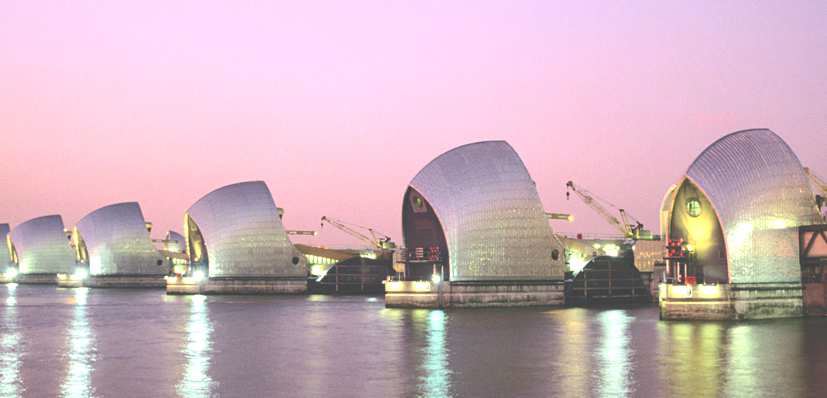
\includegraphics[width=.5\linewidth]{fig_00}
}%figues de la page de garde

\input{\repRel/Style/pagegarde_TD}
\setcounter{numques}{0}

\setlength{\columnseprule}{.1pt}

\pagestyle{fancy}
\thispagestyle{plain}

\ifprof
\vspace{5.1cm}
\else
\vspace{5.2cm}
\fi

\def\columnseprulecolor{\color{ocre}}
\setlength{\columnseprule}{0.4pt} 

%%%%%%%%%%%%%%%%%%%%%%%

\setcounter{exo}{0}



\ifprof
\else
\begin{multicols}{2}
\fi


Le comportement dynamique du rotor est étudié sur un modèle à 6 degrés de
liberté : le rotor n'étant en contact avec aucun solide, il dispose des 6 mouvements
de corps rigide. On suppose le rotor indéformable. La figure suivante montre à
gauche le rotor dans sa position nominale ($\alpha=\beta=\theta=x=y=z=0$) et à droite le
rotor dans une position quelconque. On note $A_0$ et $B_0$ les centres des paliers
magnétiques radiaux et $A$ et $B$ les points appartenant à l'arbre et confondus
avec et dans la position nominale.

\begin{center}
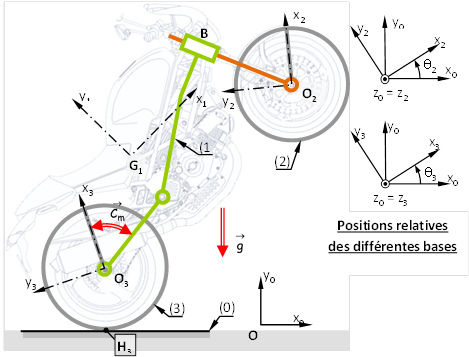
\includegraphics[width=\linewidth]{fig_01}
\end{center}



On note $O$ le milieu de $\left[ A_0 B_0\right]$ et $M$ le milieu de $\left[ A B\right]$. Bien qu'un soin très
important soit apporté à la fabrication du rotor, il est impossible d'annuler totalement
les défauts d'équilibrage. Le centre de gravité n'est donc pas exactement
situé sur l'axe $(AB)$, mais à une distance de celui-ci telle que $\vect{MG}=r_0\vect{y_3}$.

De même, la matrice d'inertie $I_{G,3}$ n'est pas parfaitement diagonale et présente
un produit d'inertie $D$ non nul. On admet toutefois que $r<<L$ et $D<<(A,B,C)$,
où $A$, $B$, $C$sont les moments d’inertie. Le mouvement du rotor, auquel on associe
le repère 3, par rapport au bâti est paramétré par les trois déplacements $(x,y,z)$
du point $M$ dans le repère $\rep{0}\repere{0}{x_0}{y_0}{z_0}$ :  $\vect{OM}=x\vect{x_0}+y\vect{y_0}+z\vect{z_0}$ ainsi que par trois rotations $\left(\alpha,\beta,\gamma\right)$ telles que :

\begin{itemize}
\item $\alpha$ paramètre la rotation d'une base $\mathcal{B}_1\base{x_0}{y_1}{z_1}$ par rapport à $\mathcal{B}_0$ autour de l'axe $\vect{x_0}$;
\item $\beta$ paramètre la rotation d'une base $\mathcal{B}_2\base{x_2}{y_1}{z_2}$ par rapport à $\mathcal{B}_1$ autour de l'axe $\vect{y_1}$;
\item $\theta$ paramètre la rotation d'une base $\mathcal{B}_3\base{x_3}{y_3}{z_2}$ par rapport à $\mathcal{B}_2$ autour de l'axe $\vect{z_2}$.
\end{itemize}

Si le rotor présente 6 degrés de liberté, il est bien évident qu'excepté la rotation
propre principale $\theta$, ces mouvements sont très petits.

En notant $\varepsilon(x)$ une fonction telle que $|\varepsilon(x)|<<|x|$, on peut écrire :
$\left\{
\begin{array}{l}
x,y,z \simeq \varepsilon(L) \\
\alpha, \beta \simeq \varepsilon(1)
\end{array}
\right.
$.

On suppose que la vitesse de rotation du rotor est constante : $\dot{\theta}=\omega$ et $\ddot{\theta}=0$.

\subsubsection*{Efforts des paliers et du moteur sur le rotor}

Pour le dimensionnement dynamique, on modélise les actions des trois paliers
magnétiques et l'action du moteur électrique sous la forme :

$\torseurstat{T}{0}{3A} = \torseurl{X_A\vect{x_0}+Y_A\vect{y_0}}{\vect{0}}{A}$, 
$\torseurstat{T}{0}{3B} = \torseurl{X_B\vect{x_0}+Y_B\vect{y_0}}{\vect{0}}{B}$,
$\torseurstat{T}{0}{3C} = \torseurl{Z_C\vect{z_0}}{\vect{0}}{C}$,
$\torseurstat{T}{\text{moteur}}{3} = \torseurl{\vect{0}}{C_m\vect{z_0}}{G}$.

Avec 
$\left\{
\begin{array}{l}
X_A\vect{x_0}+Y_A\vect{y_0} = -k\left[\vect{A_0 A}\right]_{\left(\vect{x_0},\vect{y_0} \right)} -c\left[ \vectv{A}{3}{0}\right]_{\left(\vect{x_0},\vect{y_0} \right)} \\
X_B\vect{x_0}+Y_B\vect{y_0} = -k\left[\vect{B_0 B}\right]_{\left(\vect{x_0},\vect{y_0} \right)} -c\left[ \vectv{B}{3}{0}\right]_{\left(\vect{x_0},\vect{y_0} \right)} \\
Z_C = -k \vect{C_0 C}\vect{z_0}-c\vectv{C}{3}{0}\cdot \vect{z_0}
\end{array}
\right.$
et $k=\SI{50e4}{Nm^{-1}}$ et $c=\SI{970}{Nm^{-1}s}$. La notation $\left[\vect{V}\right]_{\left(\vect{x_0},\vect{y_0} \right)}$  désigne la projection dans le plan $\left(\vect{x_0},\vect{y_0} \right)$ du vecteur $\vect{V}$.
Les actions de la pesanteur sont négligées. Le bâti est supposé être un référentiel
galiléen.


Le rotor, tel que $L=\SI{50}{mm}$, a pour masse $m=\SI{10}{kg}$, pour centre de gravité $G$
tel que $\vect{MG}=r_0\vect{y_3}$ où $r_0=\SI{0,05}{mm}$, et pour matrice d'inertie en $G$:
$\inertie{G}{3}=\matinertie{A}{A}{C}{-D}{0}{0}{B_3}$ où $A=\SI{0,08}{kg.m^2}$, $C=\SI{0,04}{kg.m^2}$ et $D=\SI{e-4}{kg.m^2}$.

On admet que $r_0\simeq \varepsilon(L)$ et $D\simeq \varepsilon(A)\simeq \varepsilon(C)$.

\begin{obj}
Proposer un modèle de comportement dynamique du rotor en phase de rotation.
\end{obj}

\question{Appliquer le Principe Fondamental de la Dynamique au rotor et l'exprimer
sous forme torsorielle.}
\ifprof
\begin{corrige}
\end{corrige}
\else
\fi



Les questions suivantes visent à déterminer le système d'équations issu de cette
équation torsorielle.

\question{Montrer que%, dans le cadre des hypothèses formulées, 
l'expression au premier ordre de la vitesse du centre de gravité $G$ du rotor par rapport au bâti
s'écrit : $\vectv{G}{3}{0}=\dot{x}\vect{x_0}+\dot{y}\vect{y_0}+\dot{z}\vect{z_0}-r_0\omega \vect{x_3}$.}
\ifprof
\begin{corrige}
\end{corrige}
\else
\fi


\question{Déterminer %, dans le cadre des hypothèses formulées, 
l'expression au premier
ordre de l'accélération du centre de gravité $G$ du rotor par rapport au
bâti 0 : $\vectg{G}{3}{0}$.}
\ifprof
\begin{corrige}
\end{corrige}
\else
\fi

On admet que par changement de base, la matrice $I_{G,3}$ s'écrit dans la base $B_2$ :
$\inertie{G}{3}=\matinertie{A}{A}{C}{-D\cos\theta}{D\sin\theta}{0}{B_2}$.



\question{Montrer que %, dans le cadre des hypothèses formulées, 
l'expression au premier ordre du moment cinétique en $G$ du rotor par rapport au bâti s'écrit :
$\vectmc{G}{3}{0}=\begin{pmatrix} A\dot{\alpha}+D\omega\sin\theta  \\ A\dot{ \beta }-D\omega\cos\theta \\ C\omega \end{pmatrix}_{B_2}$.
}
\ifprof
\begin{corrige}
\end{corrige}
\else
\fi


\question{Déterminer %, dans le cadre des hypothèses formulées, 
l'expression au premier ordre du moment dynamique en $G$ du rotor par rapport au bâti 0 : $\vectmd{G}{3}{0}$, dans la base $B_2$.}
\ifprof
\begin{corrige}
\end{corrige}
\else
\fi

Le Principe Fondamental de la Dynamique appliqué au rotor 3, réduit en $G$,
conduit alors à :
$$
\left[
\begin{array}{l}
m\ddot{x}+2c\dot{x}+2kx =-mr_0\omega^2 \sin \theta \\
m\ddot{y}+2c\dot{y}+2ky = mr_0\omega^2 \cos \theta \\
A\ddot{\alpha}+C\omega \dot{\beta }+2cL\dot{\alpha}+2kL\alpha =-D\omega^2 \cos \theta \\
A\ddot{\beta} - C\omega \dot{\alpha}+2cL\dot{\beta}+2kL\beta =-D\omega^2 \sin \theta \\
C_m=0 \\
\end{array}
\right.
$$

%\subparagraph{}
%\textit{}
%\ifprof
%\begin{corrige}
%\end{corrige}
%\else
%\fi
%
%
%\subparagraph{}
%\textit{}
%\ifprof
%\begin{corrige}
%\end{corrige}
%\else
%\fi



\ifprof
\else
\end{multicols}
\fi

